\documentclass[a4paper,12pt]{article} % добавить leqno в [] для нумерации слева
\usepackage[a4paper,top=1.3cm,bottom=2cm,left=1.5cm,right=1.5cm,marginparwidth=0.75cm]{geometry}
%%% Работа с русским языком
\usepackage{cmap}					% поиск в PDF
\usepackage{mathtext} 				% русские буквы в фомулах
\usepackage[T2A]{fontenc}			% кодировка
\usepackage[utf8]{inputenc}			% кодировка исходного текста
\usepackage[english,russian]{babel}	% локализация и переносы

\usepackage{graphicx}

\usepackage{wrapfig}
\usepackage{tabularx}

\usepackage{hyperref}
\usepackage[rgb]{xcolor}
\hypersetup{
colorlinks=true,urlcolor=blue
}
\usepackage{multirow}
\usepackage{hhline}


%%% Дополнительная работа с математикой
\usepackage{amsmath,amsfonts,amssymb,amsthm,mathtools} % AMS
\usepackage{icomma} % "Умная" запятая: $0,2$ --- число, $0, 2$ --- перечисление

%% Номера формул
\mathtoolsset{showonlyrefs=true} % Показывать номера только у тех формул, на которые есть \eqref{} в тексте.

%% Шрифты
\usepackage{euscript}	 % Шрифт Евклид
\usepackage{mathrsfs} % Красивый матшрифт

%% Свои команды
\DeclareMathOperator{\sgn}{\mathop{sgn}}

%% Перенос знаков в формулах (по Львовскому)
\newcommand*{\hm}[1]{#1\nobreak\discretionary{}
{\hbox{$\mathsurround=0pt #1$}}{}}

\begin{document}
	
	\begin{titlepage}
	\begin{center}
		{\large МОСКОВСКИЙ ФИЗИКО-ТЕХНИЧЕСКИЙ ИНСТИТУТ (НАЦИОНАЛЬНЫЙ ИССЛЕДОВАТЕЛЬСКИЙ УНИВЕРСИТЕТ)}
	\end{center}
	\begin{center}
		{\large Физтех-школа электроники, фотоники и молекулярной физики}
	\end{center}
	
	
	\vspace{4.5cm}
	{\huge
		\begin{center}
			{Лабораторная работа 4.7.2}\\
			Эффект Поккельса
		\end{center}
	}
	\vspace{2cm}
	\begin{flushright}
		{\LARGE Салтыкова Дарья \\
			\vspace{0.5cm}
			Б04-105}
	\end{flushright}
	\vspace{8cm}
	\begin{center}
		Долгопрудный 2023
	\end{center}
\end{titlepage}

\section{Введение}

\noindent
\textbf{Цель работы:} исследовать интерференцию рассеянного света,
прошедшего кристалл; наблюдать изменение характера поляризации света при наложении на кристалл электрического поля.
\medskip

\noindent \textbf{В работе используются:} гелий-неоновый лазер, поляризатор,
кристалл ниобата лития, матовая пластинка, экран, источник высоковольтного переменного и постоянного напряжения, фотодиод, осциллограф, линейка.

\medskip

\section{Теоретические сведения}

\noindent Эффект Поккельса -- изменение показателя преломления света в кристалле под действием электрического поля.\\

\medskip

\noindent Рассмотрим кристалл ниобата лития $\text{LiNbO}_3$ с цетрольноосевой симметрией вдоль оси $Z$. Для световой волны с $\mathbf{E}$ перпендикулярно $Z$ показатель преломления будет $n_o$, а для волны с $\mathbf{E}$ вдоль $Z$ -- $n_e$. В случае, когда луч света идёт под углом $\theta$ к оси, есть два значение показателя преломления $n_1$ и $n_2$: $n_1 = n_o$ для волны с $\mathbf{E}$ перпендикулярным плоскости $(\mathbf{k},\mathbf{Z})$ (обыкновенная волна) и $n_2$ для волны с $\mathbf{E}$ в этой плоскости (необыкновенная волна). В последнем случае

\begin{equation}
\dfrac{1}{n_2^2}=\dfrac{\cos^2 \theta}{n_0^2}+\dfrac{\sin^2 \theta}{n_e^2}.
\end{equation}

\begin{wrapfigure}{r}{0.5\textwidth}
\begin{center}
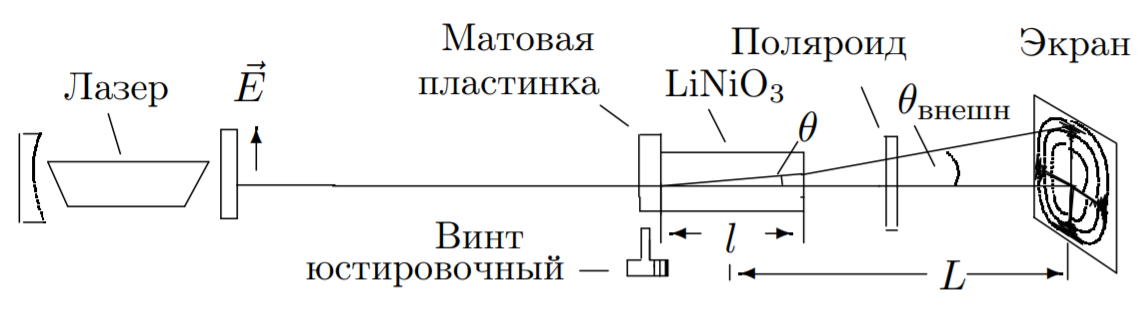
\includegraphics[width = 0.5\textwidth]{1.png}
\end{center}

\caption{Схема для наблюдения интерфереционной картины}
\end{wrapfigure}

\noindent Если перед кристаллом, помещённым между поляроидами, расположить линзу или матовую пластинку, то на экране за поляроидом мы увидим тёмные концентрические окружности -- рещультат интерфернции обыкновенной и необыкновенной волн. При повороте выходного поляроида на $90^\circ$ картина меняется с позитива на негатив (на месте светлых пятен тёмные и наоборот). В случаи, когда разрешённое направление анализатора перпендикулярно поляризации лазерного излучения, радиус тёмного кольца с номером $m$ равен

\begin{equation}
r_m^2 = \dfrac{\lambda}{l} \dfrac{(n_oL)^2}{n_0 - n_e}m,
\end{equation}

\noindent где $L$ -- расстояние от центра кристалла до экрана, $l$ -- длина кристалла.\\

\medskip

\noindent Теперь поместим кристалл в постоянное электрическое поле $E_{\text{эл}}$, направленное вдоль оси $X$, перпендикулярной $Z$. Показатель преломления для луча, распространяющего вдоль $Z$, всегда $n_o$. В плоскости $(X,Y)$ возникают два главных направления под углами $45^\circ$ к $X$ и $Y$ с показателями преломления $n_0 - \Delta n$ и $n_o + \Delta n$ (быстрая и медленная ось), причём $\Delta n = A E_{\text{эл}}$. Для поляризованного вертикально света и анализатора, пропускающего горизонтальную поляризацию, на выходе интенсивность на выходе будет иметь вид

\begin{equation}
I_{\text{вых}} = I_0 \sin^2 \left(\dfrac{\pi}{2} \dfrac{U}{U_{\lambda/2}} \right),
\end{equation}

\noindent где $U_{\lambda/2} = \frac{\lambda}{4A}\frac{d}{l}$ -- \textit{полуволновое напряжение}, $d$ -- поперечный размер кристалла.  При напряжении $U = E_{\text{эл}}d$ равном полуволновому сдвиг фаз между двумя волнами равен $\pi$, а интенсивность света на выходе максимальна. 

\section{Экспериментальная установка}

\begin{center}

  \centering
  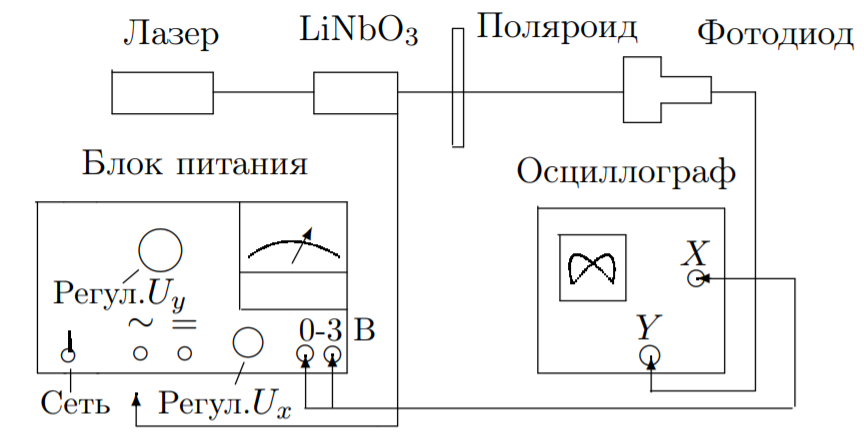
\includegraphics[scale={0.5}]{2.png}

{Рис. 2: Схема установки}

\end{center}

\noindent Оптическая часть установки
представлена на рис. 1. Свет гелий-неонового лазера, поляризованный в вертикальной плоскости, проходя сквозь матовую пластинку, рассеивается и падает на двоякопреломляющий кристалл
под различными углами. Кристалл ниобата лития с размерами
3 × 3 × 26 мм вырезан вдоль оптической оси $Z$. На экране, расположенном за скрещенным поляроидом, видна интерференционная
картина.

\medskip

\noindent Для $\lambda = 0,63 \text{ мкм}$ (длина волны гелий-неонового лазера) в ниобате лития $n_o = 2,29$.

\medskip

\noindent Убрав рассеивающую пластинку и подавая на кристалл постоянное напряжение, можно величиной напряжения влиять на поляризацию луча, вышедшего из кристалла.

\medskip

\noindent Заменив экран фотодиодом (рис. 2) и подав на кристалл переменное напряжение, можно исследовать поляризацию луча с помощью осциллографа.

\section{Ход работы}

\noindent 1. Проведем юстировку установки. Получим на экране интерференционную картину.

\medskip

\noindent 2. Измерим радуисы темных колец $r(m)$ для трех расстояний $L$ от середины кристалла до экрана. Построим графики $r^2 = f(m)$.

\medskip

\begin{table}[h!]
\begin{tabular}{lll}
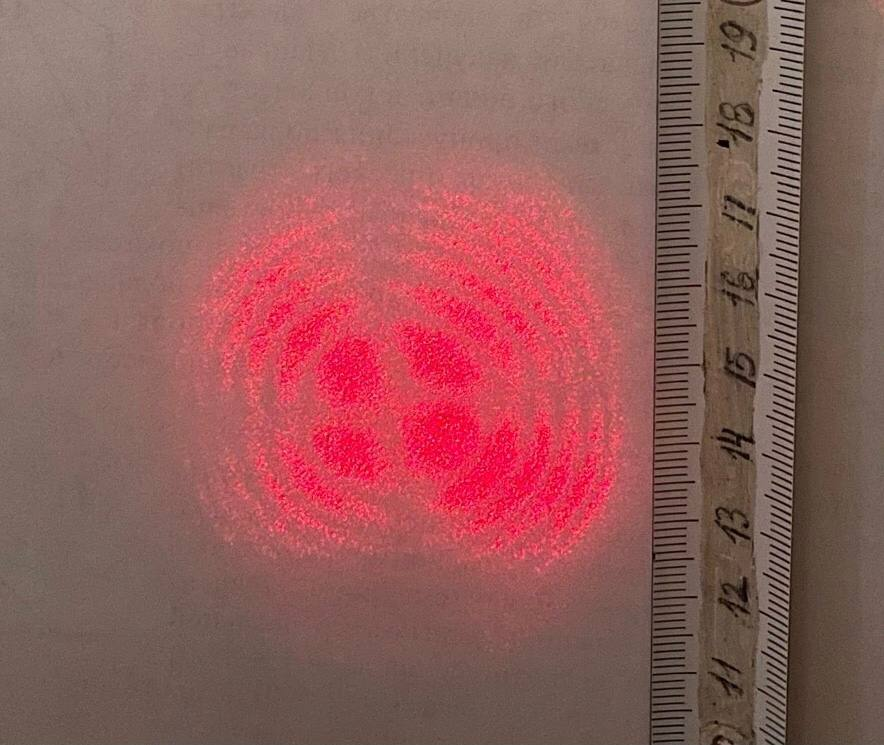
\includegraphics[width=0.3\linewidth]{l1.jpg} & 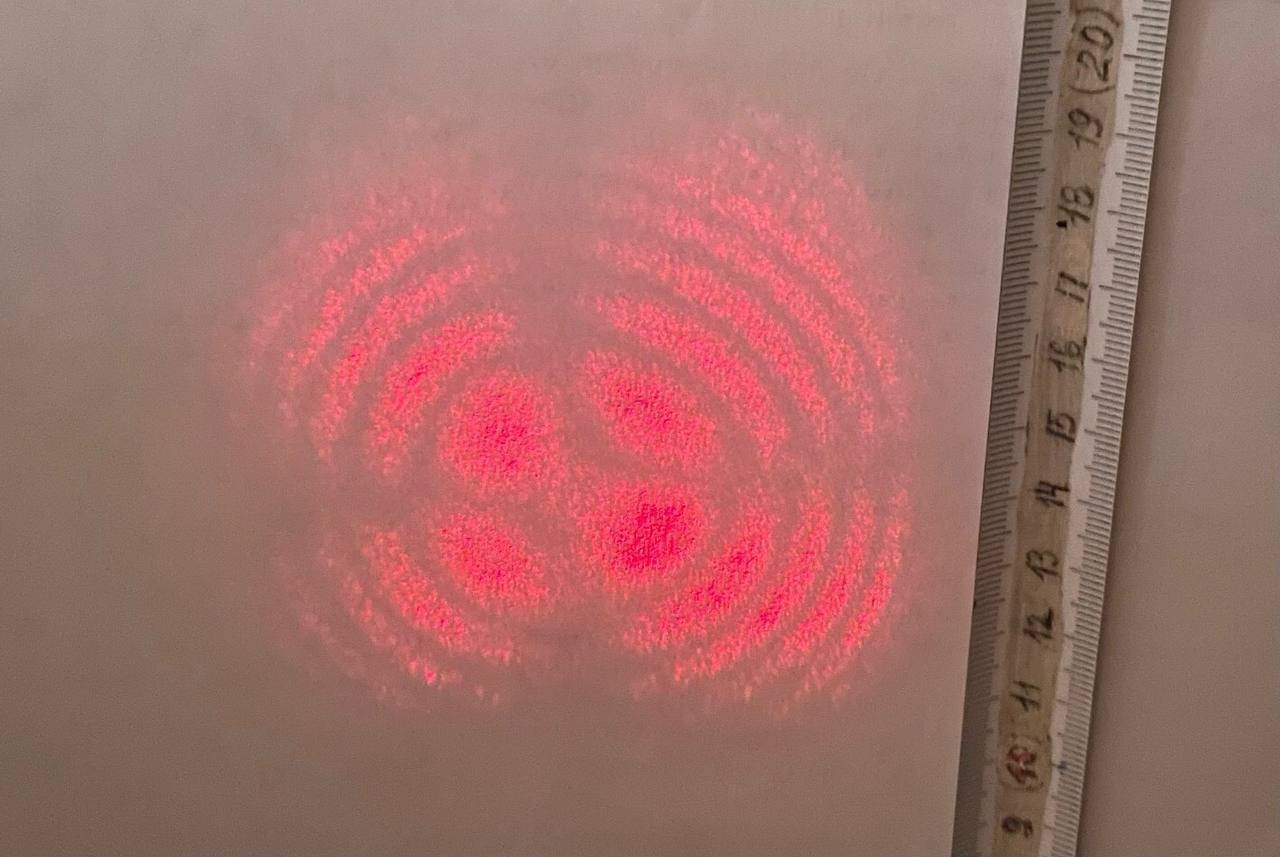
\includegraphics[width=0.3\linewidth]{l2.jpg} & 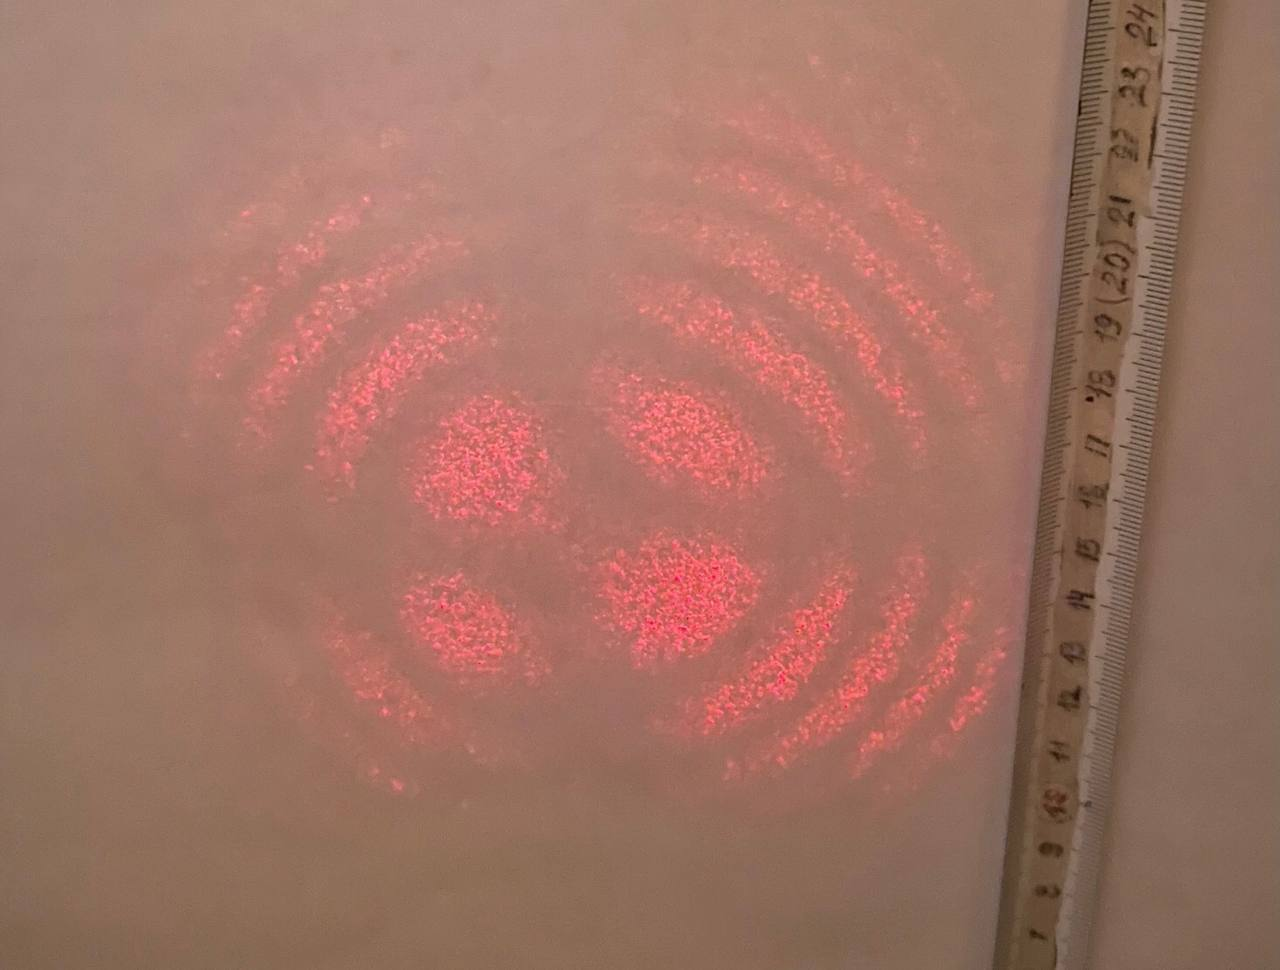
\includegraphics[width=0.3\linewidth]{l3.jpg} \\
\multicolumn{1}{c}{$L = (38,2 \pm 1,0) \text{ см}$} & \multicolumn{1}{c}{$L = (56,7 \pm 1,0) \text{ см}$} & \multicolumn{1}{c}{$L = (98,5 \pm 1,0) \text{ см}$}
\end{tabular}
\end{table}

\medskip

\begin{table}[h!]
\begin{tabular}{|lllllll}
\hline
\multicolumn{7}{|c|}{$L   = (38,2 \pm 1,0) \text{ см}$}                                                                                                                                                                 \\ \hline
\multicolumn{1}{|l|}{$m$}                        & \multicolumn{1}{l|}{1}    & \multicolumn{1}{l|}{2}    & \multicolumn{1}{l|}{3}    & \multicolumn{1}{l|}{4}    & \multicolumn{1}{l|}{5}    & \multicolumn{1}{l|}{6}   \\ \hline
\multicolumn{1}{|l|}{$r, \text{ см}$}            & \multicolumn{1}{l|}{0,9}  & \multicolumn{1}{l|}{1,4}  & \multicolumn{1}{l|}{1,8}  & \multicolumn{1}{l|}{2,1}  & \multicolumn{1}{l|}{2,4}  & \multicolumn{1}{l|}{2,7} \\ \hline
\multicolumn{1}{|l|}{$r^2, \text{ см}^2$}        & \multicolumn{1}{l|}{0,8}  & \multicolumn{1}{l|}{2,0}  & \multicolumn{1}{l|}{3,2}  & \multicolumn{1}{l|}{4,4}  & \multicolumn{1}{l|}{5,8}  & \multicolumn{1}{l|}{7,3} \\ \hline
\multicolumn{1}{|l|}{$\sigma_{r^2}, \text{ см}^2$} & \multicolumn{1}{l|}{0,4}  & \multicolumn{1}{l|}{0,4}  & \multicolumn{1}{l|}{0,3}  & \multicolumn{1}{l|}{0,3}  & \multicolumn{1}{l|}{0,7}  & \multicolumn{1}{l|}{0,8} \\ \hline
\multicolumn{6}{|c|}{$L = (56,7 \pm 1,0)   \text{ см}$}                                                                                                                                      &                          \\ \cline{1-6}
\multicolumn{1}{|l|}{$m$}                        & \multicolumn{1}{l|}{1}    & \multicolumn{1}{l|}{2}    & \multicolumn{1}{l|}{3}    & \multicolumn{1}{l|}{4}    & \multicolumn{1}{l|}{5}    &                          \\ \cline{1-6}
\multicolumn{1}{|l|}{$r, \text{ см}$}            & \multicolumn{1}{l|}{1,9}  & \multicolumn{1}{l|}{2,5}  & \multicolumn{1}{l|}{3,2}  & \multicolumn{1}{l|}{3,7}  & \multicolumn{1}{l|}{4,1}  &                          \\ \cline{1-6}
\multicolumn{1}{|l|}{$r^2, \text{ см}^2$}        & \multicolumn{1}{l|}{3,6}  & \multicolumn{1}{l|}{6,3}  & \multicolumn{1}{l|}{10,2} & \multicolumn{1}{l|}{13,7} & \multicolumn{1}{l|}{16,8} &                          \\ \cline{1-6}
\multicolumn{1}{|l|}{$\sigma_{r^2}, \text{ см}^2$} & \multicolumn{1}{l|}{0,8}  & \multicolumn{1}{l|}{0,4}  & \multicolumn{1}{l|}{0,5}  & \multicolumn{1}{l|}{1,0}  & \multicolumn{1}{l|}{1,2}  &                          \\ \cline{1-6}
\multicolumn{6}{|c|}{$L = (98,5 \pm 1,0)   \text{ см}$}                                                                                                                                      &                          \\ \cline{1-6}
\multicolumn{1}{|l|}{$m$}                        & \multicolumn{1}{l|}{1}    & \multicolumn{1}{l|}{2}    & \multicolumn{1}{l|}{3}    & \multicolumn{1}{l|}{4}    & \multicolumn{1}{l|}{5}    &                          \\ \cline{1-6}
\multicolumn{1}{|l|}{$r, \text{ см}$}            & \multicolumn{1}{l|}{3,7}  & \multicolumn{1}{l|}{4,5}  & \multicolumn{1}{l|}{5,4}  & \multicolumn{1}{l|}{6,2}  & \multicolumn{1}{l|}{6,9}  &                          \\ \cline{1-6}
\multicolumn{1}{|l|}{$r^2, \text{ см}^2$}        & \multicolumn{1}{l|}{13,7} & \multicolumn{1}{l|}{20,3} & \multicolumn{1}{l|}{29,2} & \multicolumn{1}{l|}{38,4} & \multicolumn{1}{l|}{47,6} &                          \\ \cline{1-6}
\multicolumn{1}{|l|}{$\sigma_{r^2}, \text{ см}^2$} & \multicolumn{1}{l|}{1,6}  & \multicolumn{1}{l|}{0,6}  & \multicolumn{1}{l|}{0,8}  & \multicolumn{1}{l|}{0,9}  & \multicolumn{1}{l|}{2,0}  &                          \\ \cline{1-6}
\end{tabular}
\end{table} 


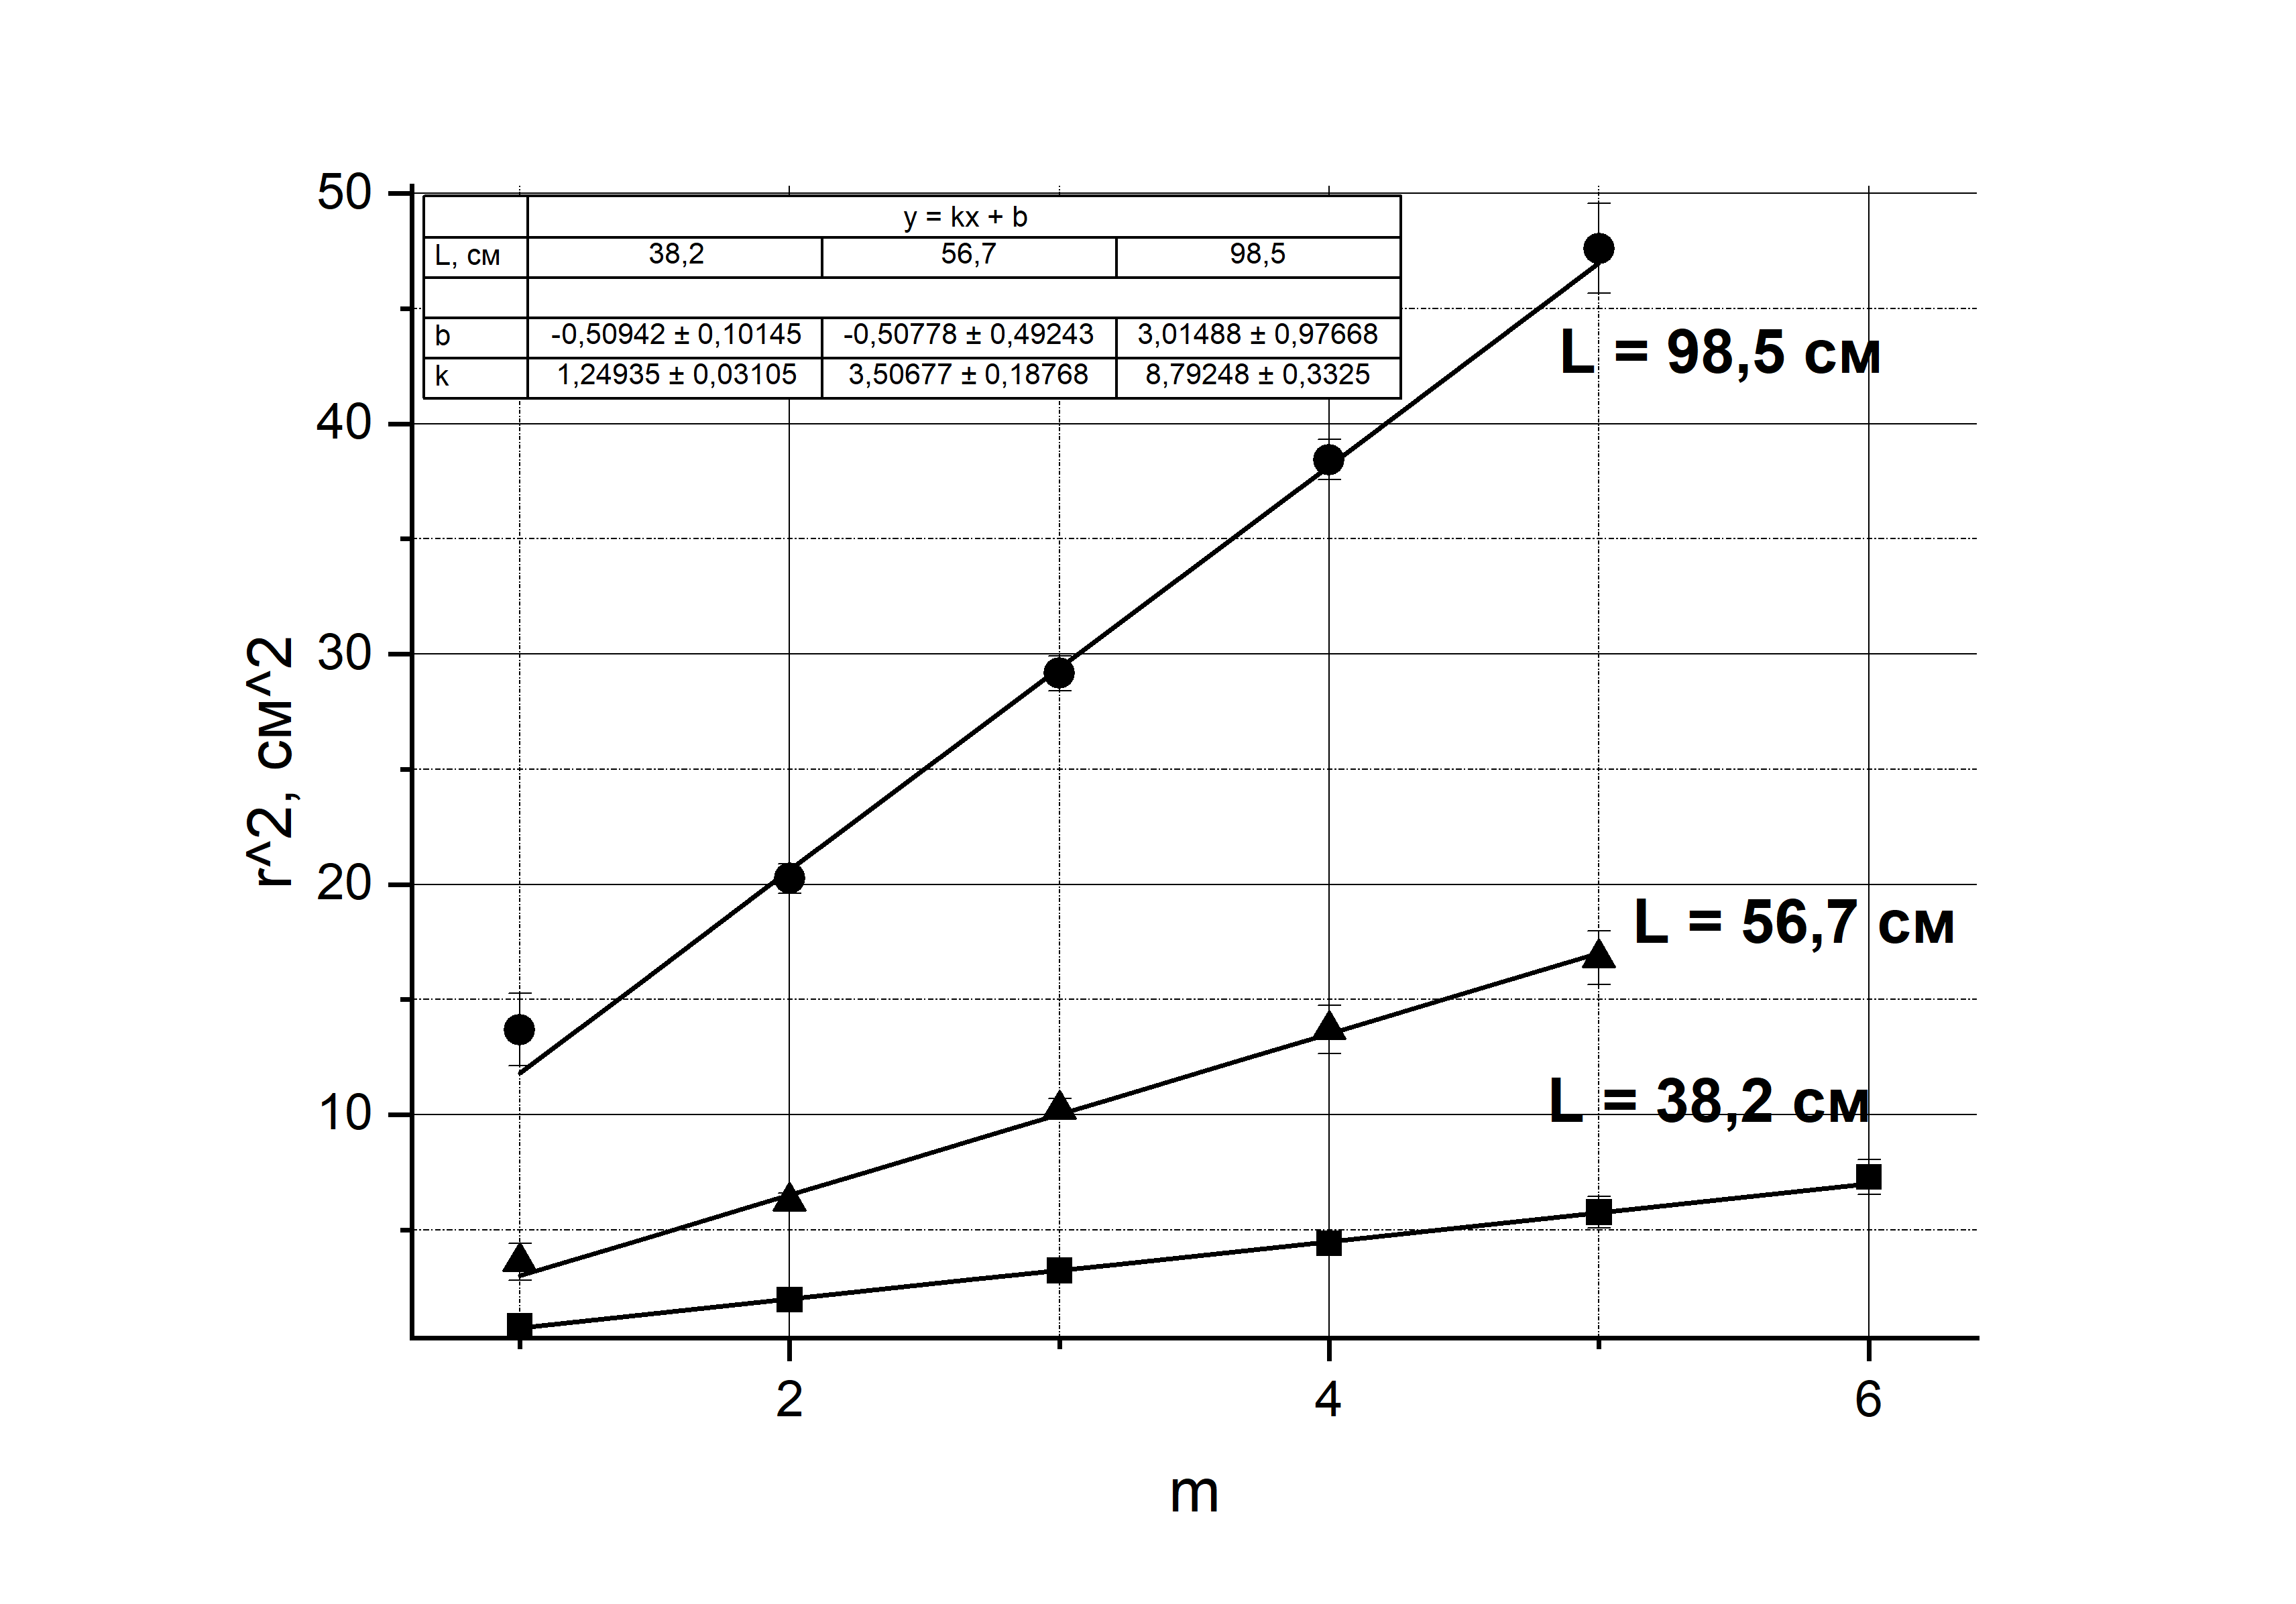
\includegraphics[width=1\linewidth]{график.png}


\medskip

\noindent По углу наклона прямой определиим двулучепреломление $(n_o - n_e)$ ниобата лития.

\medskip

\begin{table}[h!]
\begin{tabular}{|l|lll|}
\hline
$L, \text{ см}$      & \multicolumn{1}{l|}{38,2}  & \multicolumn{1}{l|}{56,7}  & 98,5  \\ \hline
$k$                  & \multicolumn{1}{l|}{1,25}  & \multicolumn{1}{l|}{3,51}  & 8,79  \\ \hline
$\sigma_k$           & \multicolumn{1}{l|}{0,03}  & \multicolumn{1}{l|}{0,19}  & 0,33  \\ \hline
$n_o - n_e$          & \multicolumn{1}{l|}{0,148} & \multicolumn{1}{l|}{0,116} & 0,140 \\ \hline
$\sigma_{n_o - n_e}$ & \multicolumn{1}{l|}{0,005} & \multicolumn{1}{l|}{0,007} & 0,005 \\ \hline
$n_o - n_e$          & \multicolumn{3}{c|}{$0,135 \pm 0,005$}                          \\ \hline
\end{tabular}
\end{table}

\medskip

\noindent 3. Убедимся ещё раз, что направление лазерного луча совпадает с направлением на центр интерференционной картины и уберём матовую пластинку. Подключим разъём блока питания на постоянно напряжение, установим регулятор напряжения на минимум и включим блок питания в сеть.

\medskip

\noindent При нулевом напряжении наблюдается минимум интенсиности излучения на экране. Постепенно увеличивая его, получим напряжение, соответстующее максимуму интенсивности $U_{\lambda/2} = (375 \pm 15) \text{ В}$. Погрешность принимаем равной одному делению - 15 В.

\medskip

\noindent 4. Подадим на кристалл четвертьволновое напряжение. Вращая анализатор наблюдаем, что яркость пятна не зависит от угла поворота анализатора - поляризация круговая.

\medskip

\noindent 5. Установим вместо экрана фотодиод (Рис. 2) и подключим его
к Y-входу осциллографа. Убрав напряжение до нуля, переключим разъём с постоянного на переменное напряжение.

\medskip

\noindent Постепенно повышая напряжение на кристалле, наблюдаем на
экране осциллографа фигуры Лиссажу, соответствующие зависимости $I_\text{вых}(U)$ для скрещенных поляризаций лазера
и анализатора. 

{$U_{\lambda/2} = (390 \pm 15) \text{ В}$}. 

\noindent Продолжая увеличивать напряжение получаем:

\[U_\lambda = (780 \pm 15) \text{ В} \qquad U_{3\lambda/2} = (1140 \pm 15) \text{ В}\]


\begin{table}[h!]
\begin{tabular}{lll}
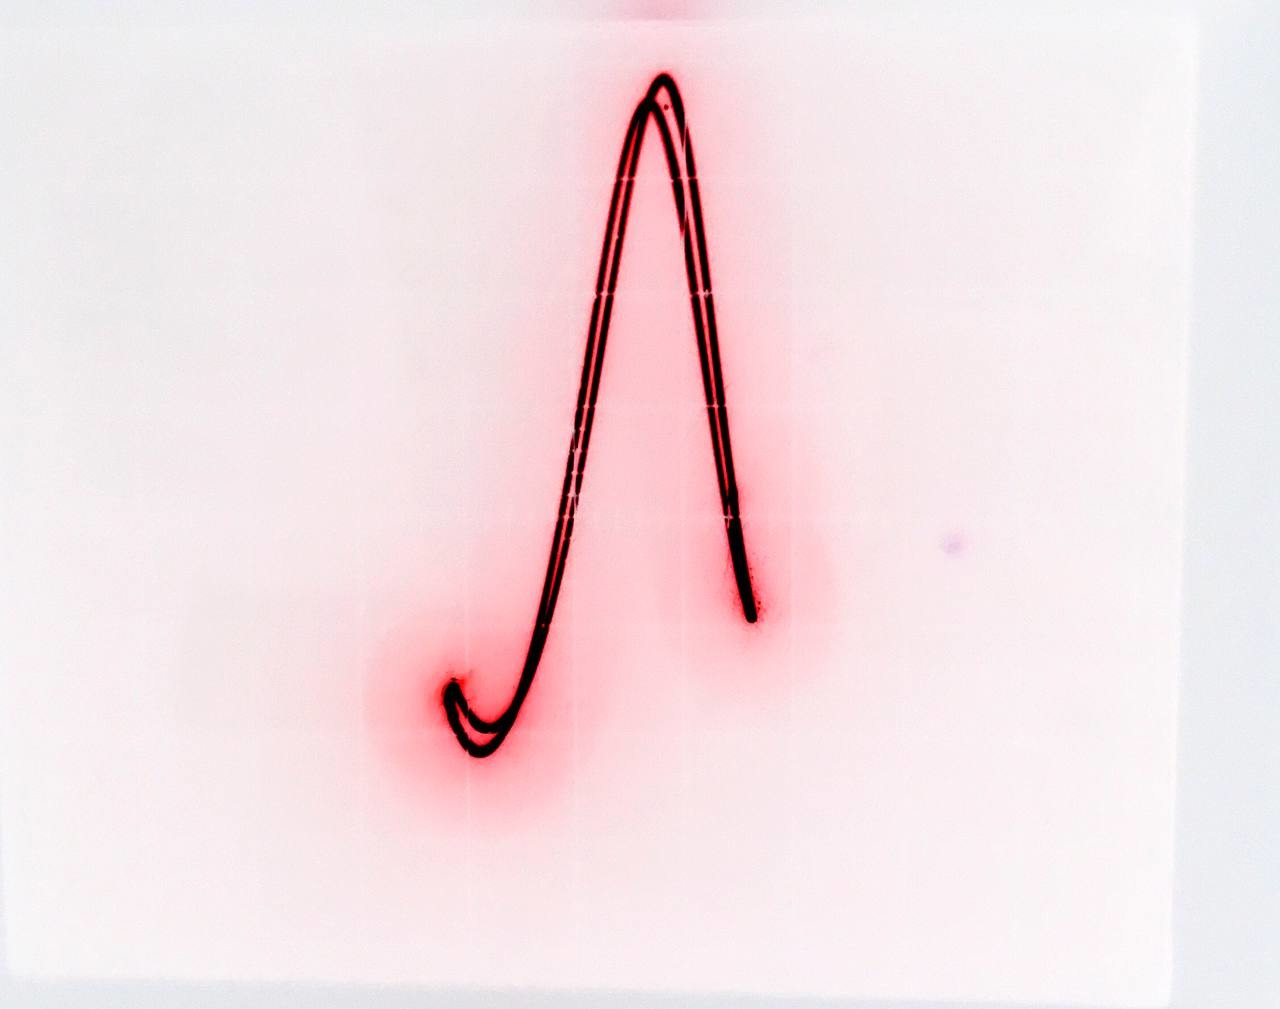
\includegraphics[width=0.3\linewidth]{1-2.jpg} & 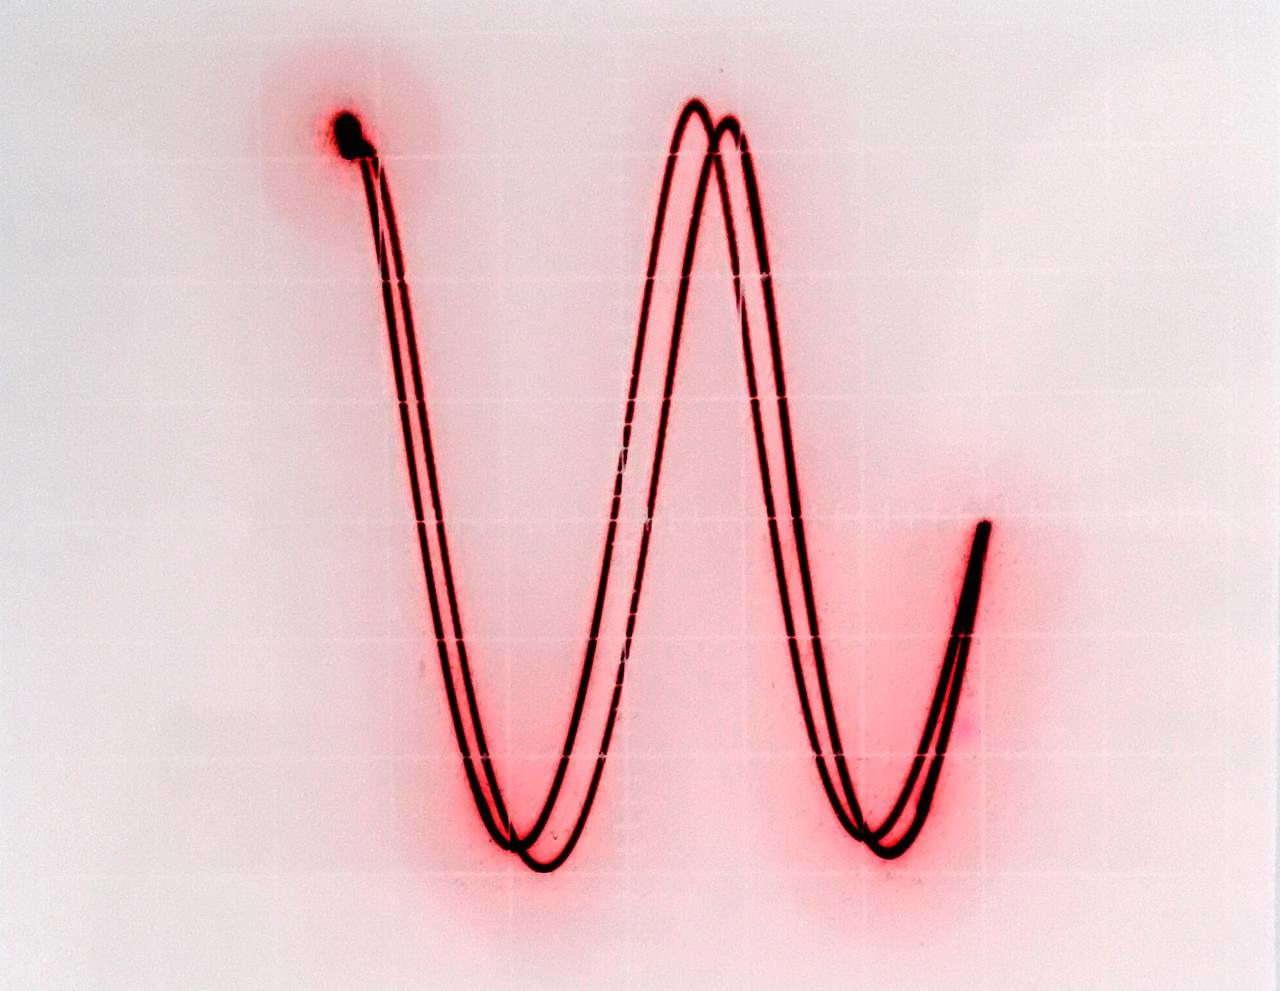
\includegraphics[width=0.3\linewidth]{1-0.jpg} & 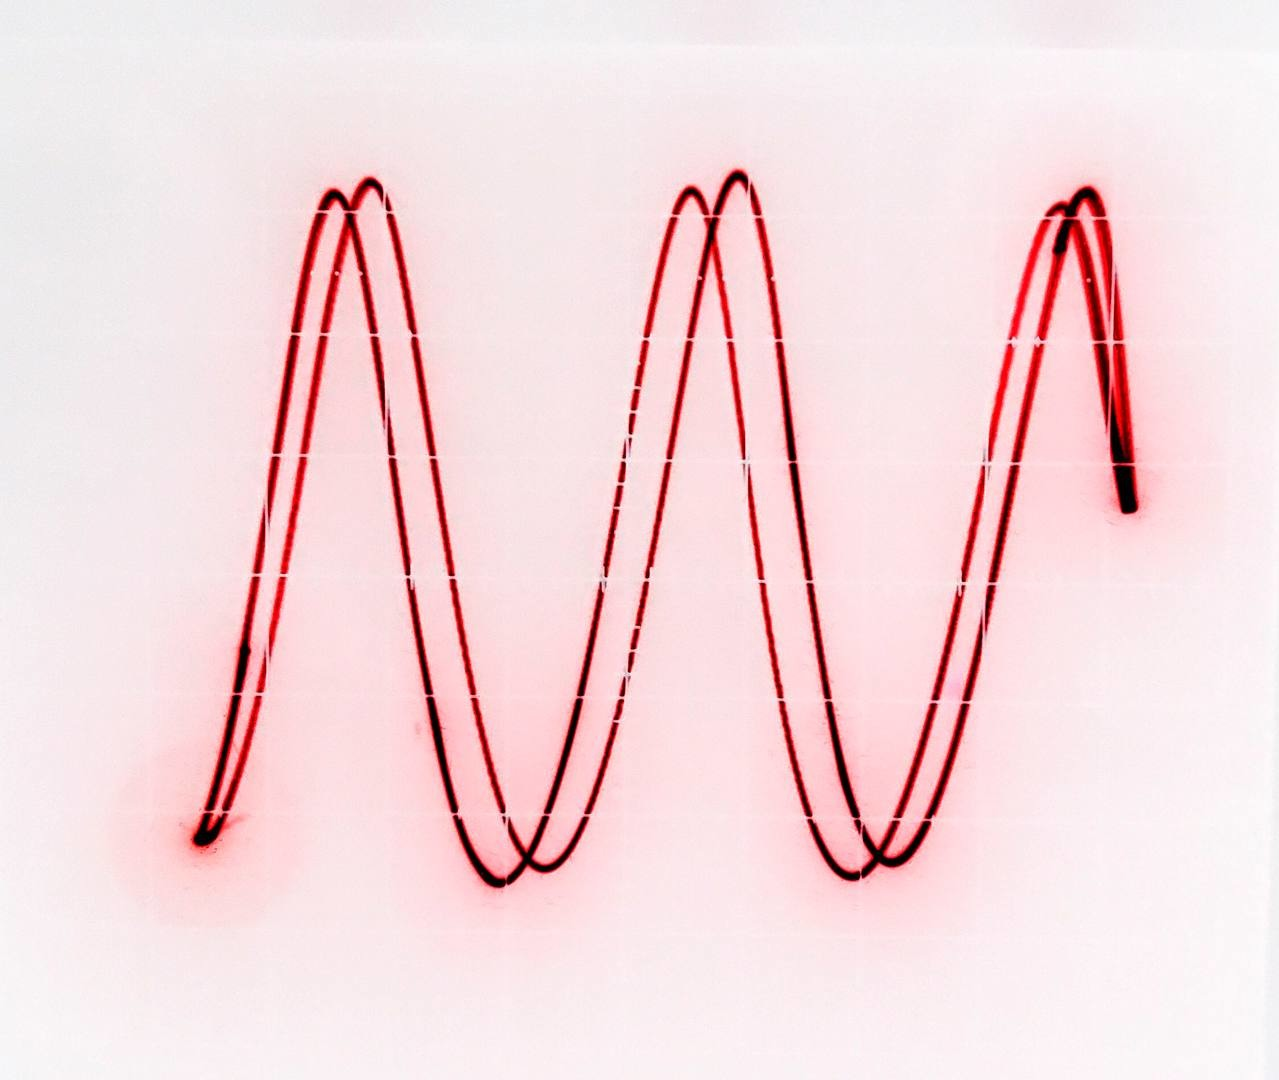
\includegraphics[width=0.3\linewidth]{3-2.jpg} \\
\multicolumn{1}{c}{$U_{\lambda/2}$}  & \multicolumn{1}{c}{$U_{\lambda}$} & \multicolumn{1}{c}{$U_{3\lambda/2}$}
\end{tabular}
\end{table}

\medskip

\noindent При переходе к параллельным поляризациям картина инвертируется.

\medskip

\begin{figure}[!h]
 	\centering
 	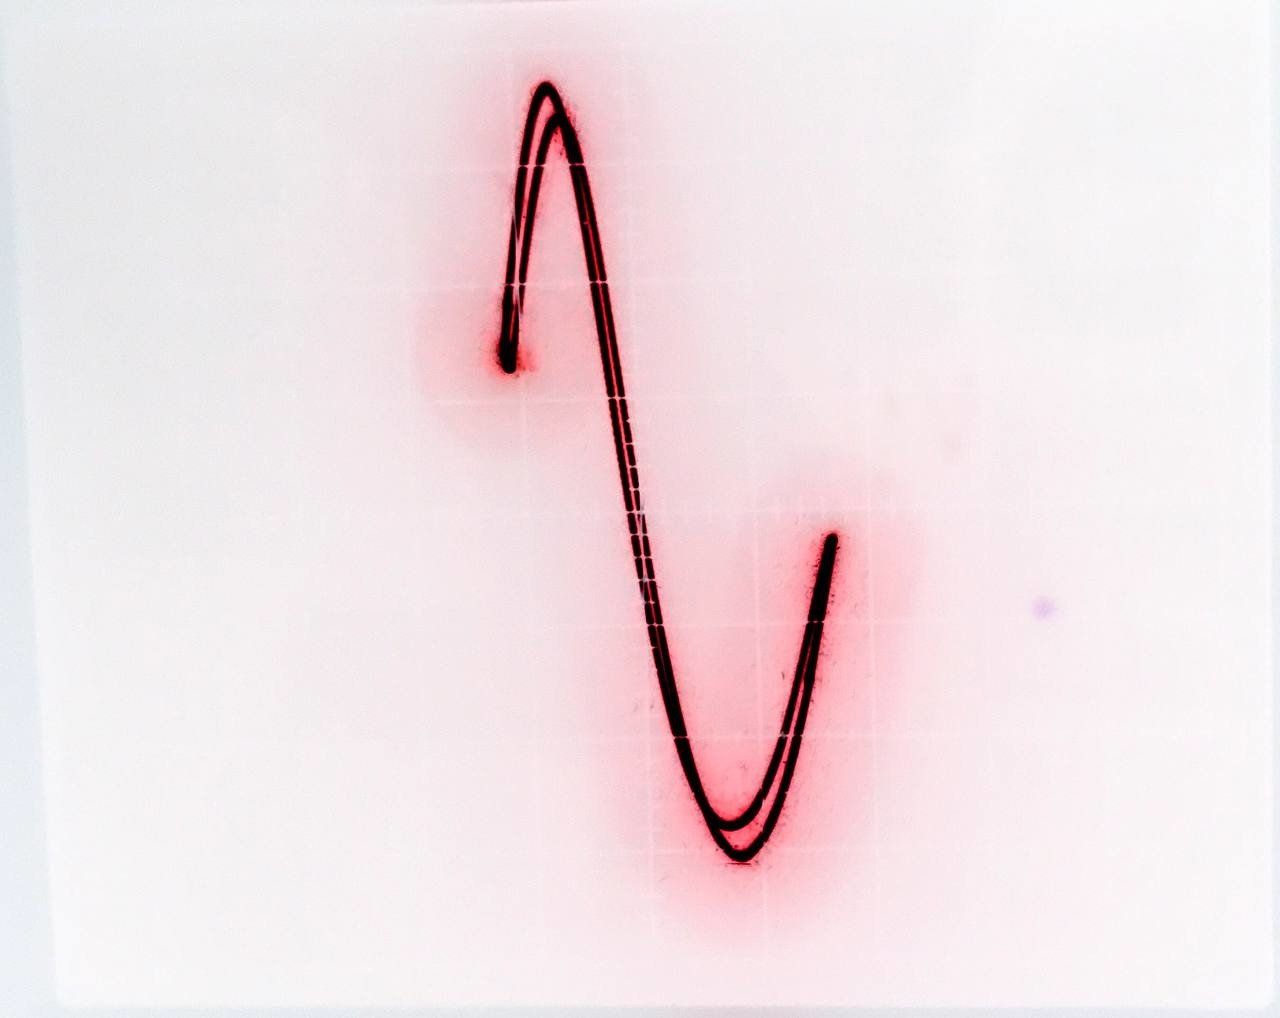
\includegraphics[width=0.3\linewidth]{inv.jpg}
 
 \end{figure}


\section{Вывод}

\medskip

\noindent В ходе работы

\medskip

\noindent 1) была определиена разность показателей преломления $n_o - n_e = 0,135 \pm 0,005$ путем измерения радиусов интерференционных колец. Табличное значение этой величины составляет $(n_o - n_e)_\text{табл} = 0,09$. Основной вклад в ошибку внесла неточность при определении радиуса колец.

\medskip

\noindent 2) при подаче на кристалл постоянного четвертьволнового напряжения, был получен свет, поляризованный по кругу. 

\medskip

\noindent 3) было определено полуволновое напряжение кристалла при постоянном напряжении:

$$U_{\lambda/2} = (375 \pm 15) \text{ В,}$$

\noindent а также полуволновое и кратные ему напряжения по фигурам Лиссажу: 

\[U_{\lambda/2} = (390 \pm 15) \text{ В} \qquad U_\lambda = (780 \pm 15) \text{ В} \qquad U_{3\lambda/2} = (1140 \pm 15) \text{ В.}\]

\end{document}